%
% xkcd.tex -- XKCD
%
% (c) 2021 Prof Dr Andreas Müller, OST Ostschweizer Fachhochschule
%
\bgroup
\begin{frame}[t]
\setlength{\abovedisplayskip}{5pt}
\setlength{\belowdisplayskip}{5pt}
\frametitle{Minimaler Weg}
\vspace{-60pt}
\begin{columns}[t,onlytextwidth]
\begin{column}{0.58\textwidth}
\begin{center}
\begin{tikzpicture}[>=latex]
\node at (0,0) {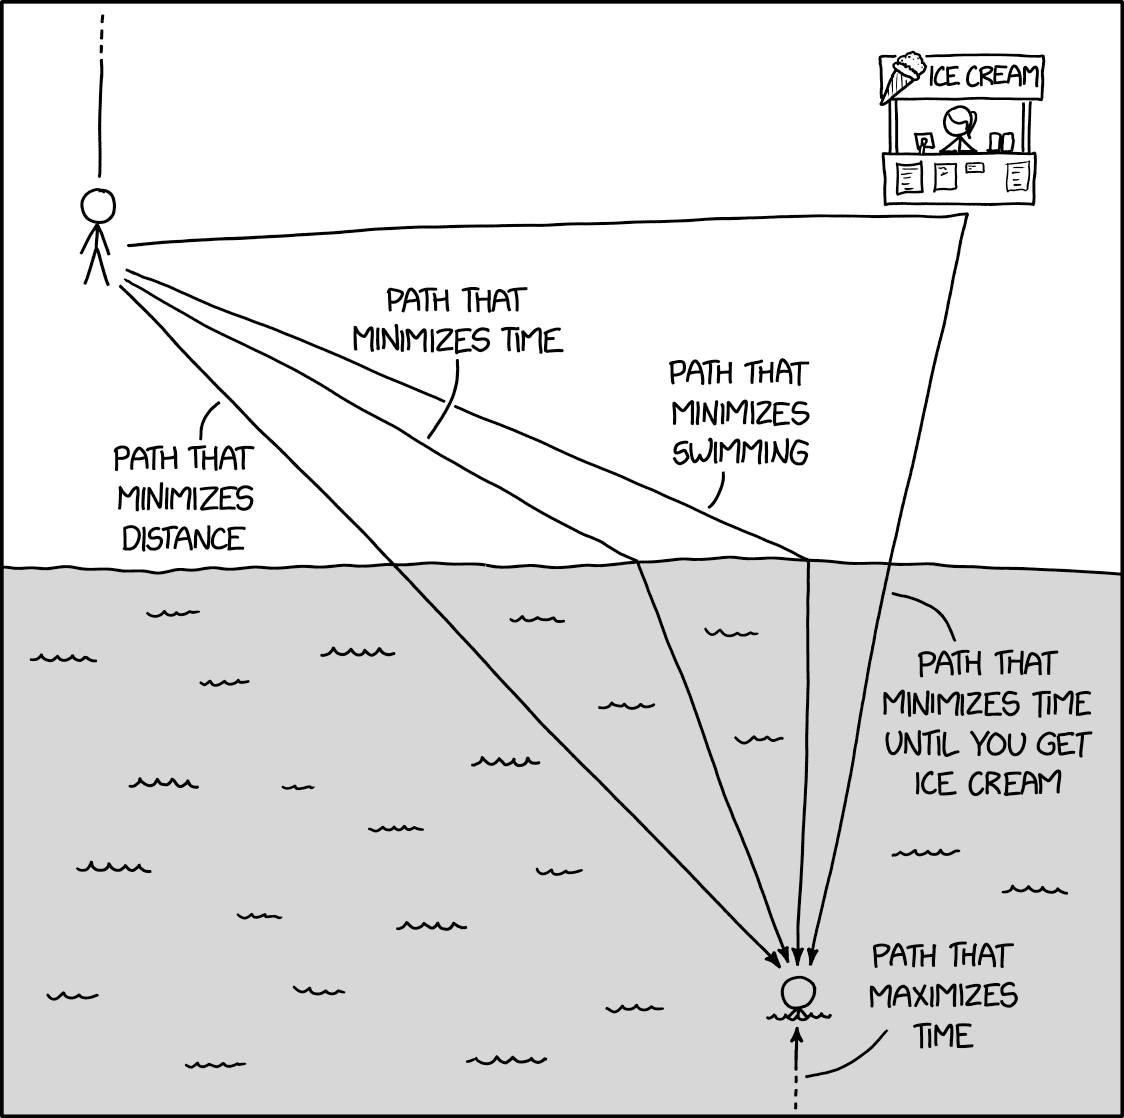
\includegraphics[width=\textwidth]{../slides/0/xkcd.jpg}};
\uncover<2->{
	\fill[color=green,opacity=0.5] (-3.21,2.44) circle[radius=0.1];
	\fill[color=green,opacity=0.5] (1.64,-3.0) circle[radius=0.1];
}
\uncover<3>{
	\draw[color=red,line width=4pt,opacity=0.5]
		(-3.06,1.9) -- (1.5,-2.82);
}
\uncover<4>{
	\draw[color=red,line width=4pt,opacity=0.5]
		(-3.05,1.94) -- (0.52,-0.01) -- (1.57,-2.80);
}
\uncover<5>{
	\draw[color=red,line width=4pt,opacity=0.5]
		(-3.04,2.01) -- (1.72,-0.01) -- (1.62,-2.82);
}
\uncover<1-6>{
	\fill[color=white] (2.1,2.42) rectangle (3.4,3.6);
}
\uncover<7>{
	\draw[color=red,line width=4pt,opacity=0.5]
		(-3.03,2.18) -- (2.82,2.41) -- (1.70,-2.82);
}
\uncover<6>{
	\draw[->,color=red,line width=4pt,opacity=0.5]
		(-3.20,2.58) -- +(0,1.3);
	\draw[<-,color=red,line width=4pt,opacity=0.5]
		(1.62,-3.1) -- +(0,-1.4);
}
\end{tikzpicture}
\end{center}
\end{column}
\begin{column}{0.48\textwidth}
\end{column}
\end{columns}
\end{frame}
\egroup
